\subsection{Datengrundlage}
Als Datengrundlage wird das öffentlich verfügbare CMB Bild der ESA Planck 
Mission in Rektangularprojektion \cite{cmb_public_equirectangular} 
verwendet. Dieses ist in Abbildung \ref{fig:cmb-rectangular} zu sehen.

\begin{figure}
	\centering
	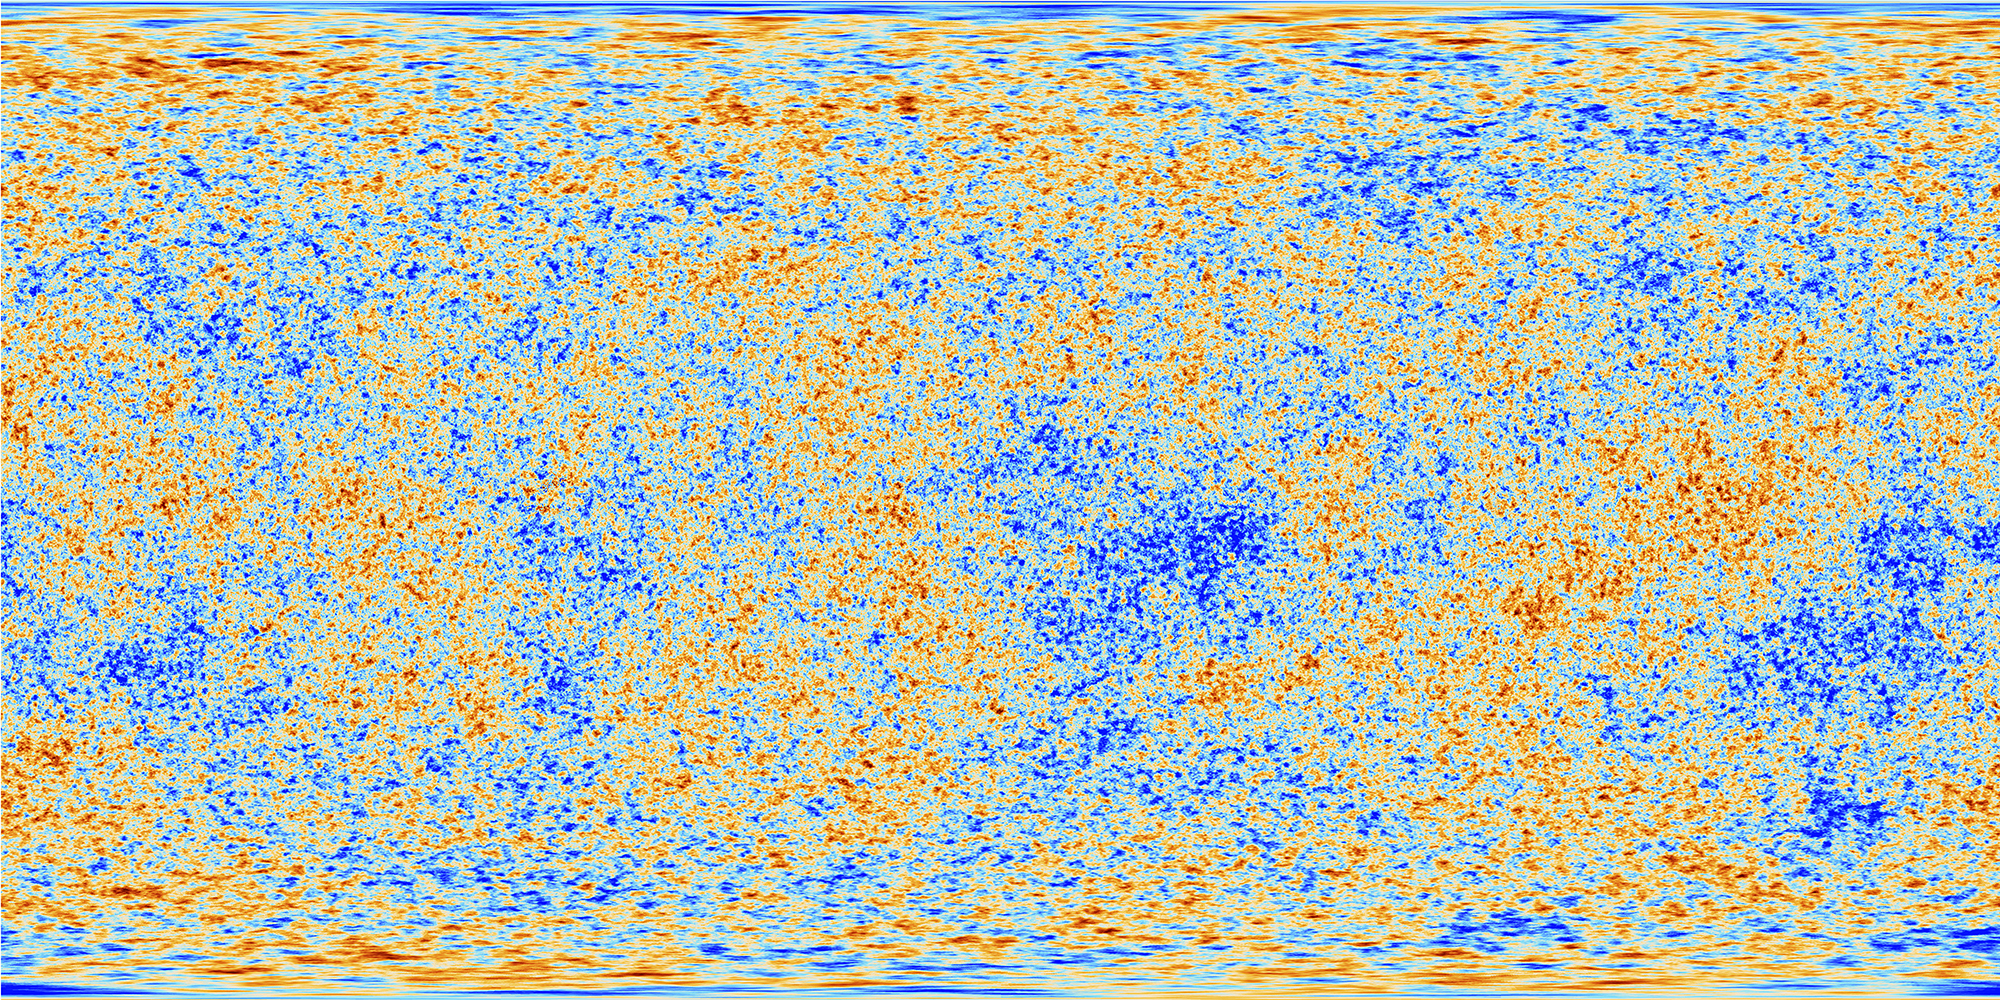
\includegraphics[width=\linewidth]{cmb/images/CMB_Planck_E.jpg}
	\caption{Das generierte Bild des CMBs in Rektangularprojektion der ESA 
		Planck mission. Es liefert die Datengrundlage für die weitere Analyse.}
	\label{fig:cmb-rectangular}
\end{figure}

Für die Analyse werden drei verschiedene Auflösungen des Bildes untersucht. 
Diese reichen von 2K (2000x1000 Pixel) über 4K (4000x2000 Pixel) bis hin zu 12K 
(12572x6286 Pixel). Diese Resultate der einzelnen Analysen finden sich im 
Abschnitt \ref{subsec:cmb:results}.



\begin{figure}
	\centering
	\includegraphics[width=\linewidth]{cmb/images/color-strip-full.png}
	\caption{Farbverlauf der für die Codierung des CMB Bildes der ESA Planck 
		Mission verwendet wurde.}
	\label{fig:color-strip-orig}
\end{figure}

\begin{figure}
	\centering
	\includegraphics[width=\linewidth]{cmb/converter/rgb-graph.pdf}
	\caption{RGB Profil des in Abbildung~\ref{fig:color-strip-orig} 
		verwendeten Farbverlaufs.}
	\label{fig:color-strip-orig-rgb}
\end{figure}

\begin{figure}
	\centering
	\includegraphics[width=\linewidth]{cmb/converter/converter-function-strip.png}
	\caption{Der für die erste Analye verwendete Farbverlauf.}
	\label{fig:color-strip}
\end{figure}

\begin{figure}
	\centering
	\includegraphics[width=\linewidth]{cmb/converter/converter-function.pdf}
	\caption{RGB Profil des in Abbildung~\ref{fig:color-strip} 
		verwendeten Farbverlaufs.}
	\label{fig:color-strip-rgb}
\end{figure}